\documentclass[12pt,a4paper]{article}
\usepackage[utf8]{inputenc}
\usepackage[T1]{fontenc}
\usepackage{geometry}
\usepackage{graphicx}
\usepackage{xcolor}
\usepackage{titlesec}
\usepackage{fancyhdr}
\usepackage{listings}
\usepackage{amsmath}
\usepackage{amsfonts}
\usepackage{hyperref}
\usepackage{booktabs}
\usepackage{array}
\usepackage{enumitem}
\usepackage{float}
\usepackage{caption}
\usepackage{subcaption}
\usepackage{tikz}
\usepackage{tcolorbox}
\usepackage{setspace}

% Set up geometry
\geometry{
    top=2.5cm,
    bottom=2.5cm,
    left=2.5cm,
    right=2.5cm
}

% Define colors matching the provided image
\definecolor{cse404green}{RGB}{76, 175, 80}
\definecolor{orangetitle}{RGB}{255, 152, 0}
\definecolor{bluepurple}{RGB}{121, 85, 178}
\definecolor{tealblue}{RGB}{69, 90, 100}
\definecolor{lightgray}{RGB}{245, 245, 245}

% Custom title formatting
\titleformat{\section}
{\normalfont\Large\bfseries\color{bluepurple}}
{\thesection}{1em}{}

\titleformat{\subsection}
{\normalfont\large\bfseries\color{tealblue}}
{\thesubsection}{1em}{}

% Set up hyperref
\hypersetup{
    colorlinks=true,
    linkcolor=bluepurple,
    filecolor=magenta,
    urlcolor=tealblue,
    pdftitle={Call of Duty Weapon Knowledgebase Report},
    pdfauthor={Sharif Md. Yousuf}
}

% Custom code listing style
\lstset{
    backgroundcolor=\color{lightgray},
    basicstyle=\ttfamily\small,
    breaklines=true,
    frame=single,
    numbers=left,
    numberstyle=\tiny\color{gray},
    keywordstyle=\color{blue},
    commentstyle=\color{green!60!black},
    stringstyle=\color{red}
}

\begin{document}

% Front page design matching the provided image
\begin{titlepage}
    \centering

    % CSE 404 Header Box
    \vspace*{2cm}
    {\Huge\bfseries\color{white}
        \colorbox{cse404green}{\makebox[8cm][c]{CSE 404}}
    }

    \vspace{1cm}

    % Main Title
    {\Huge\bfseries\color{orangetitle}
        Artificial Intelligence and\\
        Expert Systems Lab
    }

    \vspace{2cm}

    % Technical Report Title
    {\Large\bfseries\color{tealblue}
        Technical Report on \\ Call of Duty Weapon Knowledgebase
    }

    \vspace{0.5cm}

    {\large\color{bluepurple}
        Submission Date: 2/8/2025
    }

    \vspace{3cm}

    % Two column layout for submission info
    \begin{minipage}[t]{0.45\textwidth}
        \centering
        {\Large\bfseries\color{white}
            \colorbox{bluepurple}{\makebox[5cm][c]{Submitted by}}
        }

        \vspace{0.5cm}

        {\large\bfseries Name: Sharif Md. Yousuf}

        \vspace{0.3cm}

        {\large Registration ID:\@ 22101128}

        \vspace{0.3cm}

        {\large Section: C-2}

        \vspace{0.3cm}

        {\large Semester: 4-1}

        \vspace{0.3cm}

        {\large Session: Spring 2025}
    \end{minipage}
    \hfill
    \begin{minipage}[t]{0.45\textwidth}
        \centering
        {\Large\bfseries\color{white}
            \colorbox{tealblue}{\makebox[5cm][c]{Submitted to}}
        }

        \vspace{0.5cm}

        {\large\bfseries Bidita Sarkar Diba}

        \vspace{0.3cm}

        {\large Lecturer}

        \vspace{0.3cm}

        {\large Department of Computer}

        \vspace{0.3cm}

        {\large Science \& Engineering}

        \vspace{0.3cm}

        {\large University of Asia Pacific}
    \end{minipage}

    \vfill

\end{titlepage}

% Table of Contents
\tableofcontents
\newpage

% Main Content
\section{Problem Title}

\textbf{Call of Duty Weapon Knowledgebase: A Comprehensive Prolog Implementation for Modeling Gaming Arsenal Systems and Recursive Progression Analysis}

This project implements a sophisticated Prolog knowledgebase that models the
extensive weapon ecosystem from the Call of Duty franchise, spanning over two
decades of gaming history from 2003 to 2024. The system captures not only basic
weapon attributes but also complex attachment systems, game mechanics, and
recursive progression chains that mirror the intricate unlock systems found in
modern gaming.

\section{Problem Description}

The gaming industry, particularly first-person shooter games like Call of Duty,
features incredibly complex weapon systems that involve hundreds of weapons,
attachments, and progression mechanics. Understanding these systems requires
organizing vast amounts of interconnected data and implementing logical rules
that can handle recursive relationships and complex queries.

\subsection{Domain Complexity}

The Call of Duty franchise presents a perfect case study for knowledge
representation due to its:

\begin{itemize}
    \item \textbf{Temporal Span}: 18 games released over 21 years (2003-2024)
    \item \textbf{Weapon Diversity}: 121 unique weapons across 8 different categories
    \item \textbf{Attachment Systems}: 49 attachments with compatibility matrices
    \item \textbf{Game Mechanics}: 26 different mechanics spanning 5 categories
    \item \textbf{Progression Systems}: Complex unlock chains requiring recursive analysis
\end{itemize}

\subsection{Technical Challenges}

Implementing this knowledgebase presented several technical challenges:

\begin{enumerate}
    \item \textbf{Recursive Progression Modeling}: Weapons unlock in chains where accessing advanced weapons requires progressing through intermediate ones. This necessitated implementing recursive rules that could traverse these chains efficiently while avoiding infinite loops.

    \item \textbf{Multi-Dimensional Classification}: Each weapon belongs to multiple classification systems simultaneously (era, type, role, performance tier), requiring flexible rule systems that could handle overlapping categories.

    \item \textbf{Attachment Compatibility}: With 121 weapons and 49 attachments, the compatibility matrix contains thousands of potential combinations, each with different effectiveness ratings.

    \item \textbf{Optimization Algorithms}: Finding optimal weapon builds requires analyzing multiple criteria simultaneously and recommending combinations that maximize specific attributes like damage, accuracy, or stealth.
\end{enumerate}

\subsection{Knowledge Representation Goals}

The primary objectives were to create a system that could:

\begin{itemize}
    \item Store and retrieve complex weapon data efficiently
    \item Handle recursive queries for progression analysis
    \item Provide intelligent recommendations for weapon builds
    \item Support statistical analysis across different game eras
    \item Enable flexible querying for research and analysis purposes
\end{itemize}

\section{Tools and Languages Used}

\textbf{SWI-Prolog 9.0+\@} served as the core implementation language for this knowledgebase project. Prolog was selected for its excellent support for recursive rule definition, built-in unification and backtracking mechanisms, and powerful constraint solving capabilities. The declarative nature of Prolog made it ideal for representing complex weapon relationships and implementing sophisticated recursive algorithms for progression analysis.

\textbf{Visual Studio Code} was used as the primary development environment, enhanced with Prolog extensions that provided syntax highlighting, error detection, and integrated debugging capabilities. The IDE facilitated efficient code organization and version control integration through Git, enabling systematic project development and documentation management.

\textbf{LaTeX\@} was employed for comprehensive report generation, allowing for professional document formatting and mathematical notation support. The typesetting system enabled the creation of well-structured technical documentation with proper formatting for code listings, diagrams, and academic referencing.

\textbf{Mermaid} diagram language was utilized for creating architectural visualizations and system structure diagrams. This tool provided an efficient way to represent the complex relationships between different components of the knowledgebase in a clear, visual format that enhances understanding of the system architecture.

\textbf{Testing and Validation Tools} included custom test suites with over 50 test cases, validation scripts for data integrity checking, and performance benchmarking utilities for recursive query optimization. These tools ensured the reliability and correctness of the implemented system.

\section{Diagram/Figure}

The knowledgebase architecture follows a layered approach with clear separation
of concerns, as illustrated in Figure 1. The system is organized into multiple
interconnected layers that handle different aspects of the weapon ecosystem.

% Note: Use -- for en-dash or --- for em-dash in LaTeX for proper dash usage.

\begin{figure}[H]
    \centering
    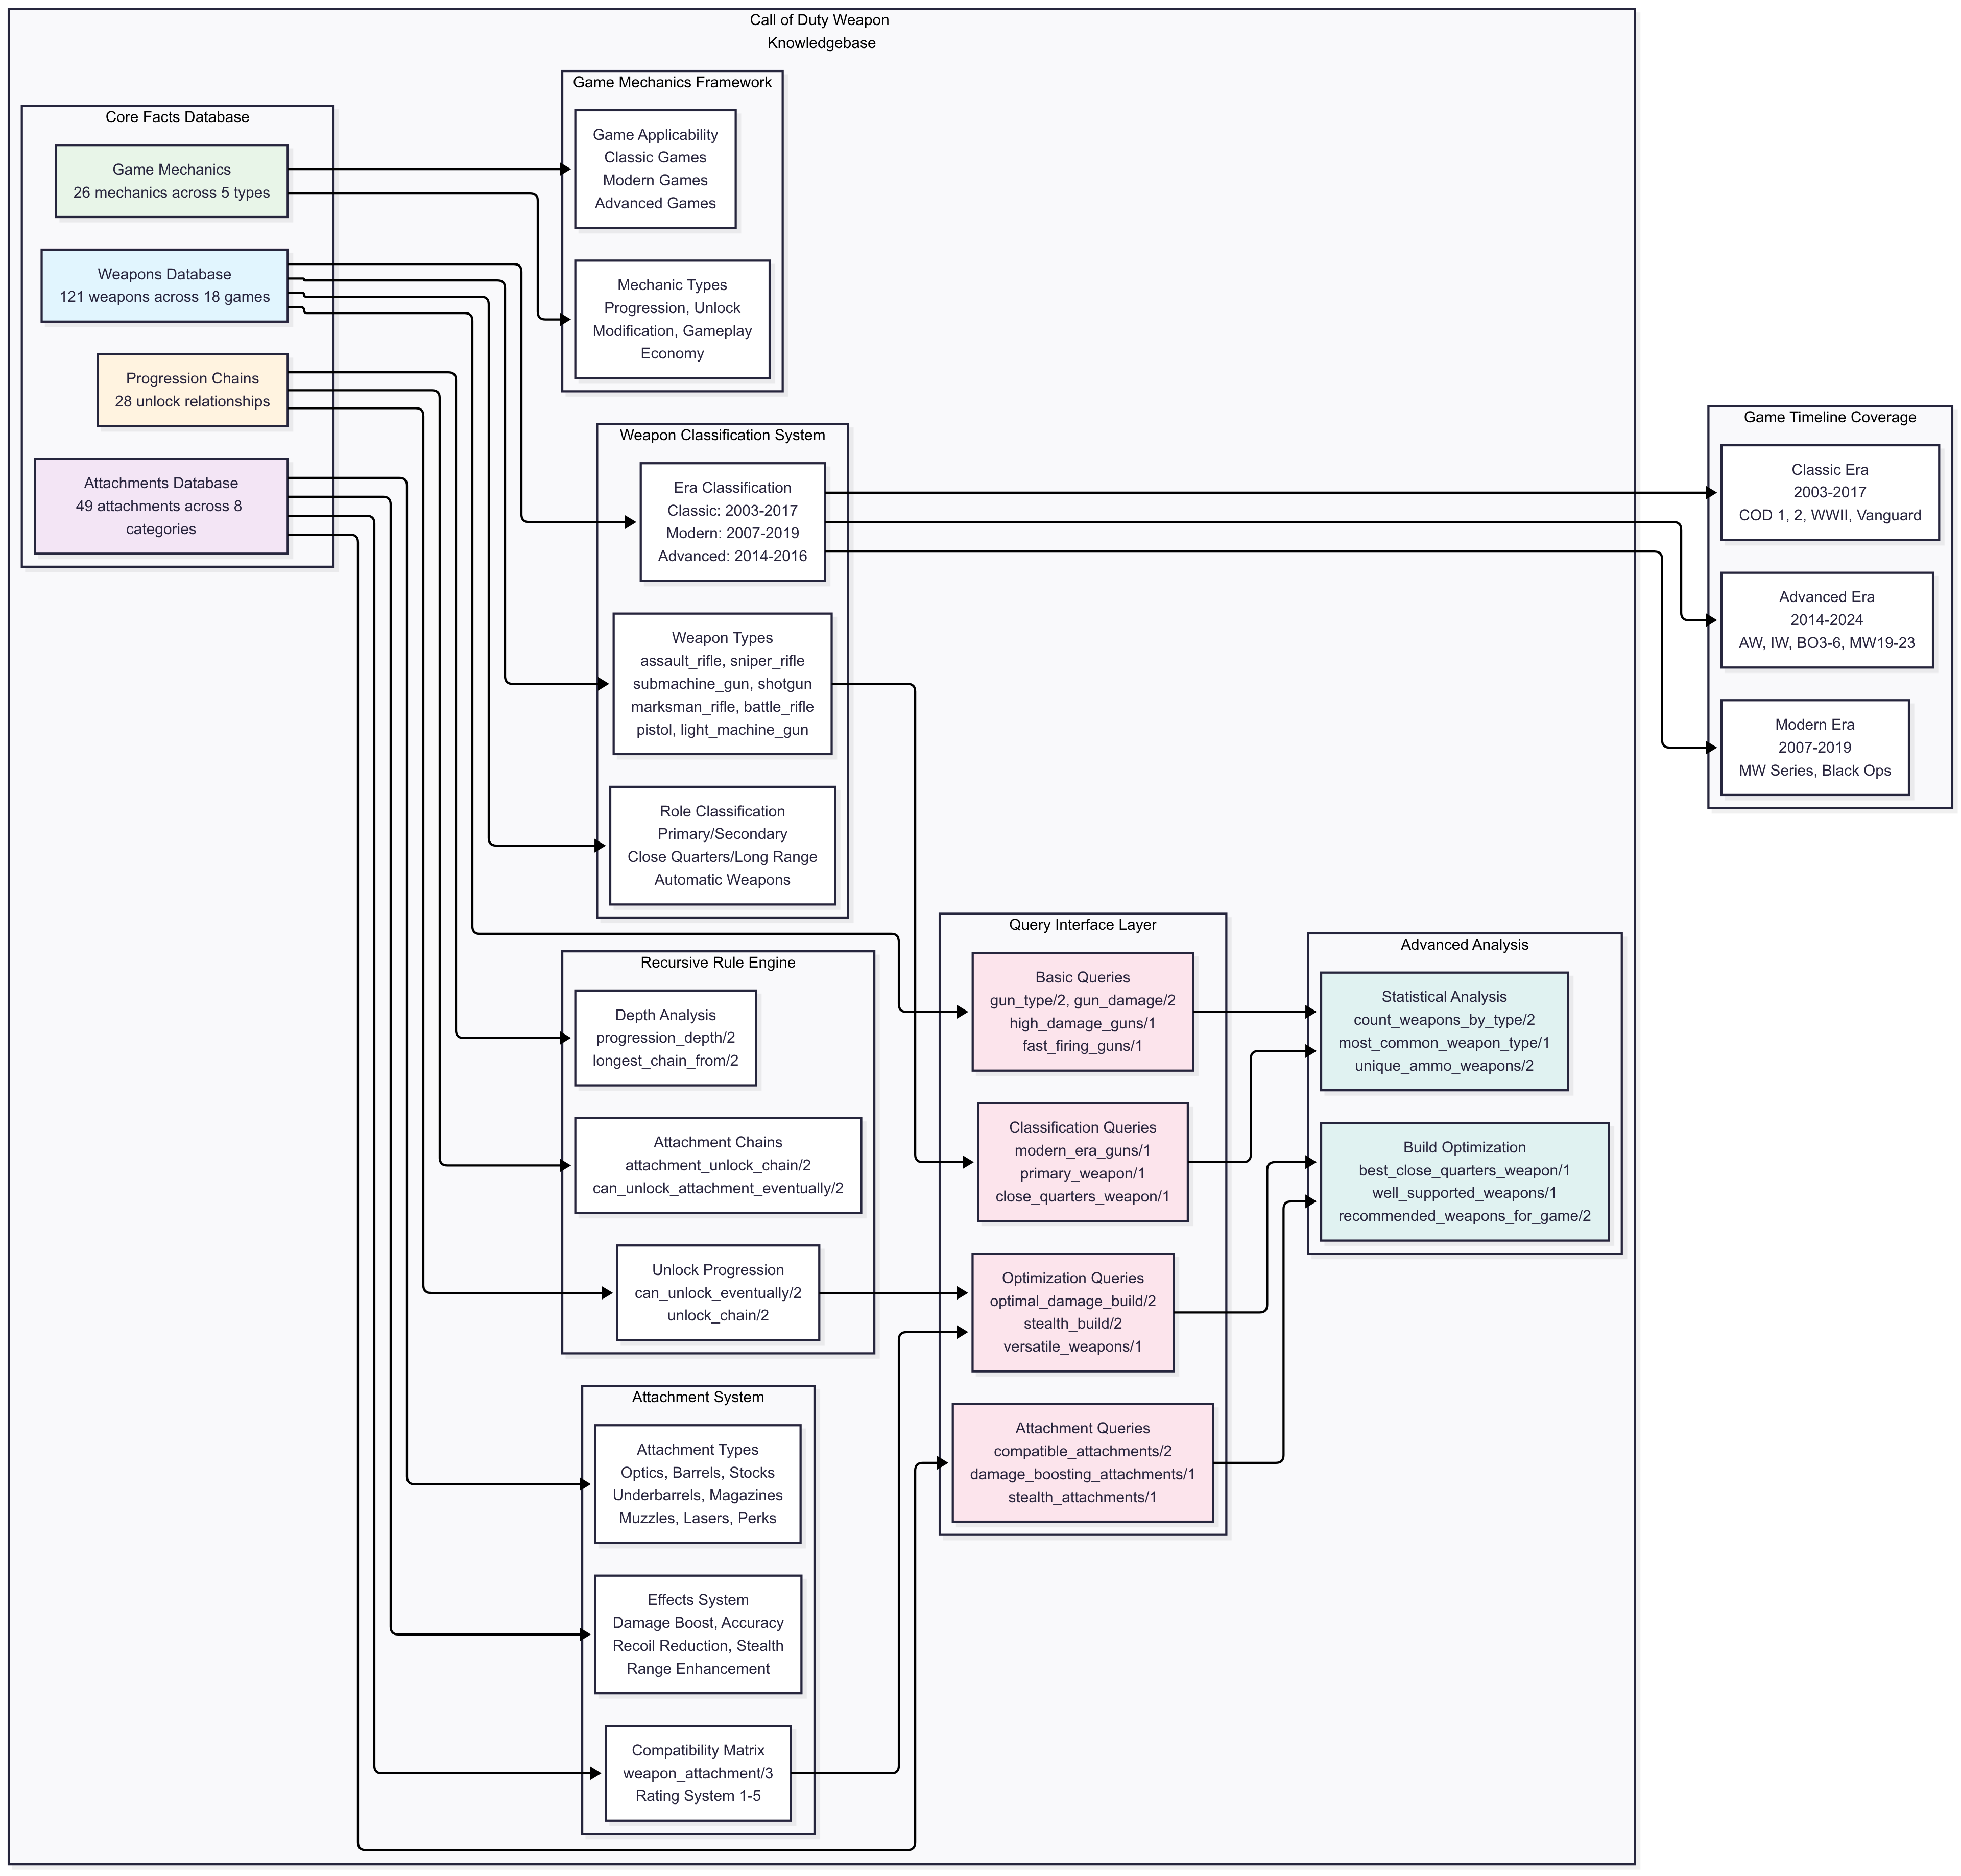
\includegraphics[width=0.8\textwidth]{../diagrams/knowledgebase-diagram-vertical.png}
    \caption{Call of Duty Weapon Knowledgebase System Architecture}
\end{figure}

\subsection{System Architecture Components}

\textbf{Core Facts Database Layer} forms the foundation with four primary databases: Weapons Database containing 121 weapon facts with detailed attributes, Attachments Database with 49 attachments across 8 categories, Game Mechanics encompassing 26 mechanics across 5 types, and Progression Chains managing 28 unlock relationships for recursive analysis.

\textbf{Weapon Classification System} provides multi-dimensional categorization including weapon types (assault rifles, sniper rifles, submachine guns, shotguns, marksman rifles, battle rifles, pistols, light machine guns), era classification spanning Classic (2003-2017), Modern (2007-2019), and Advanced (2014-2024) periods, and role classification distinguishing between primary/secondary weapons and close quarters/long range applications.

\textbf{Attachment System} manages attachment types across optics, barrels, stocks, underbarrels, magazines, muzzles, lasers, and perks, implements an effects system for damage boost, accuracy enhancement, recoil reduction, stealth capabilities, and range enhancement, and maintains a compatibility matrix using weapon\_attachment/3 predicate with a 1-5 rating system.

\textbf{Recursive Rule Engine} implements sophisticated algorithms for unlock progression analysis through predicates like can\_unlock\_eventually/2 and unlock\_chain/2, provides depth analysis capabilities with progression\_depth/2 and longest\_chain\_from/2, and manages attachment progression chains via attachment\_unlock\_chain/2 and can\_unlock\_attachment\_eventually/2.

\textbf{Query Interface Layer} offers comprehensive access through 30+ predicates organized into basic queries (gun\_type/2, gun\_damage/2), classification queries (modern\_era\_guns/1, primary\_weapon/1), attachment queries (compatible\_attachments/2, stealth\_attachments/1), and optimization queries (optimal\_damage\_build/2, versatile\_weapons/1).

\textbf{Advanced Analysis Layer} provides statistical analysis capabilities for counting weapons by type and identifying patterns, along with build optimization algorithms for recommending optimal weapon configurations for specific scenarios.

\subsection{Weapon Classification Hierarchy}

The weapon classification system is organized in a hierarchical structure that categorizes weapons by type, family relationships, and evolutionary progression, as shown in Figure 2.

\begin{figure}[H]
    \centering
    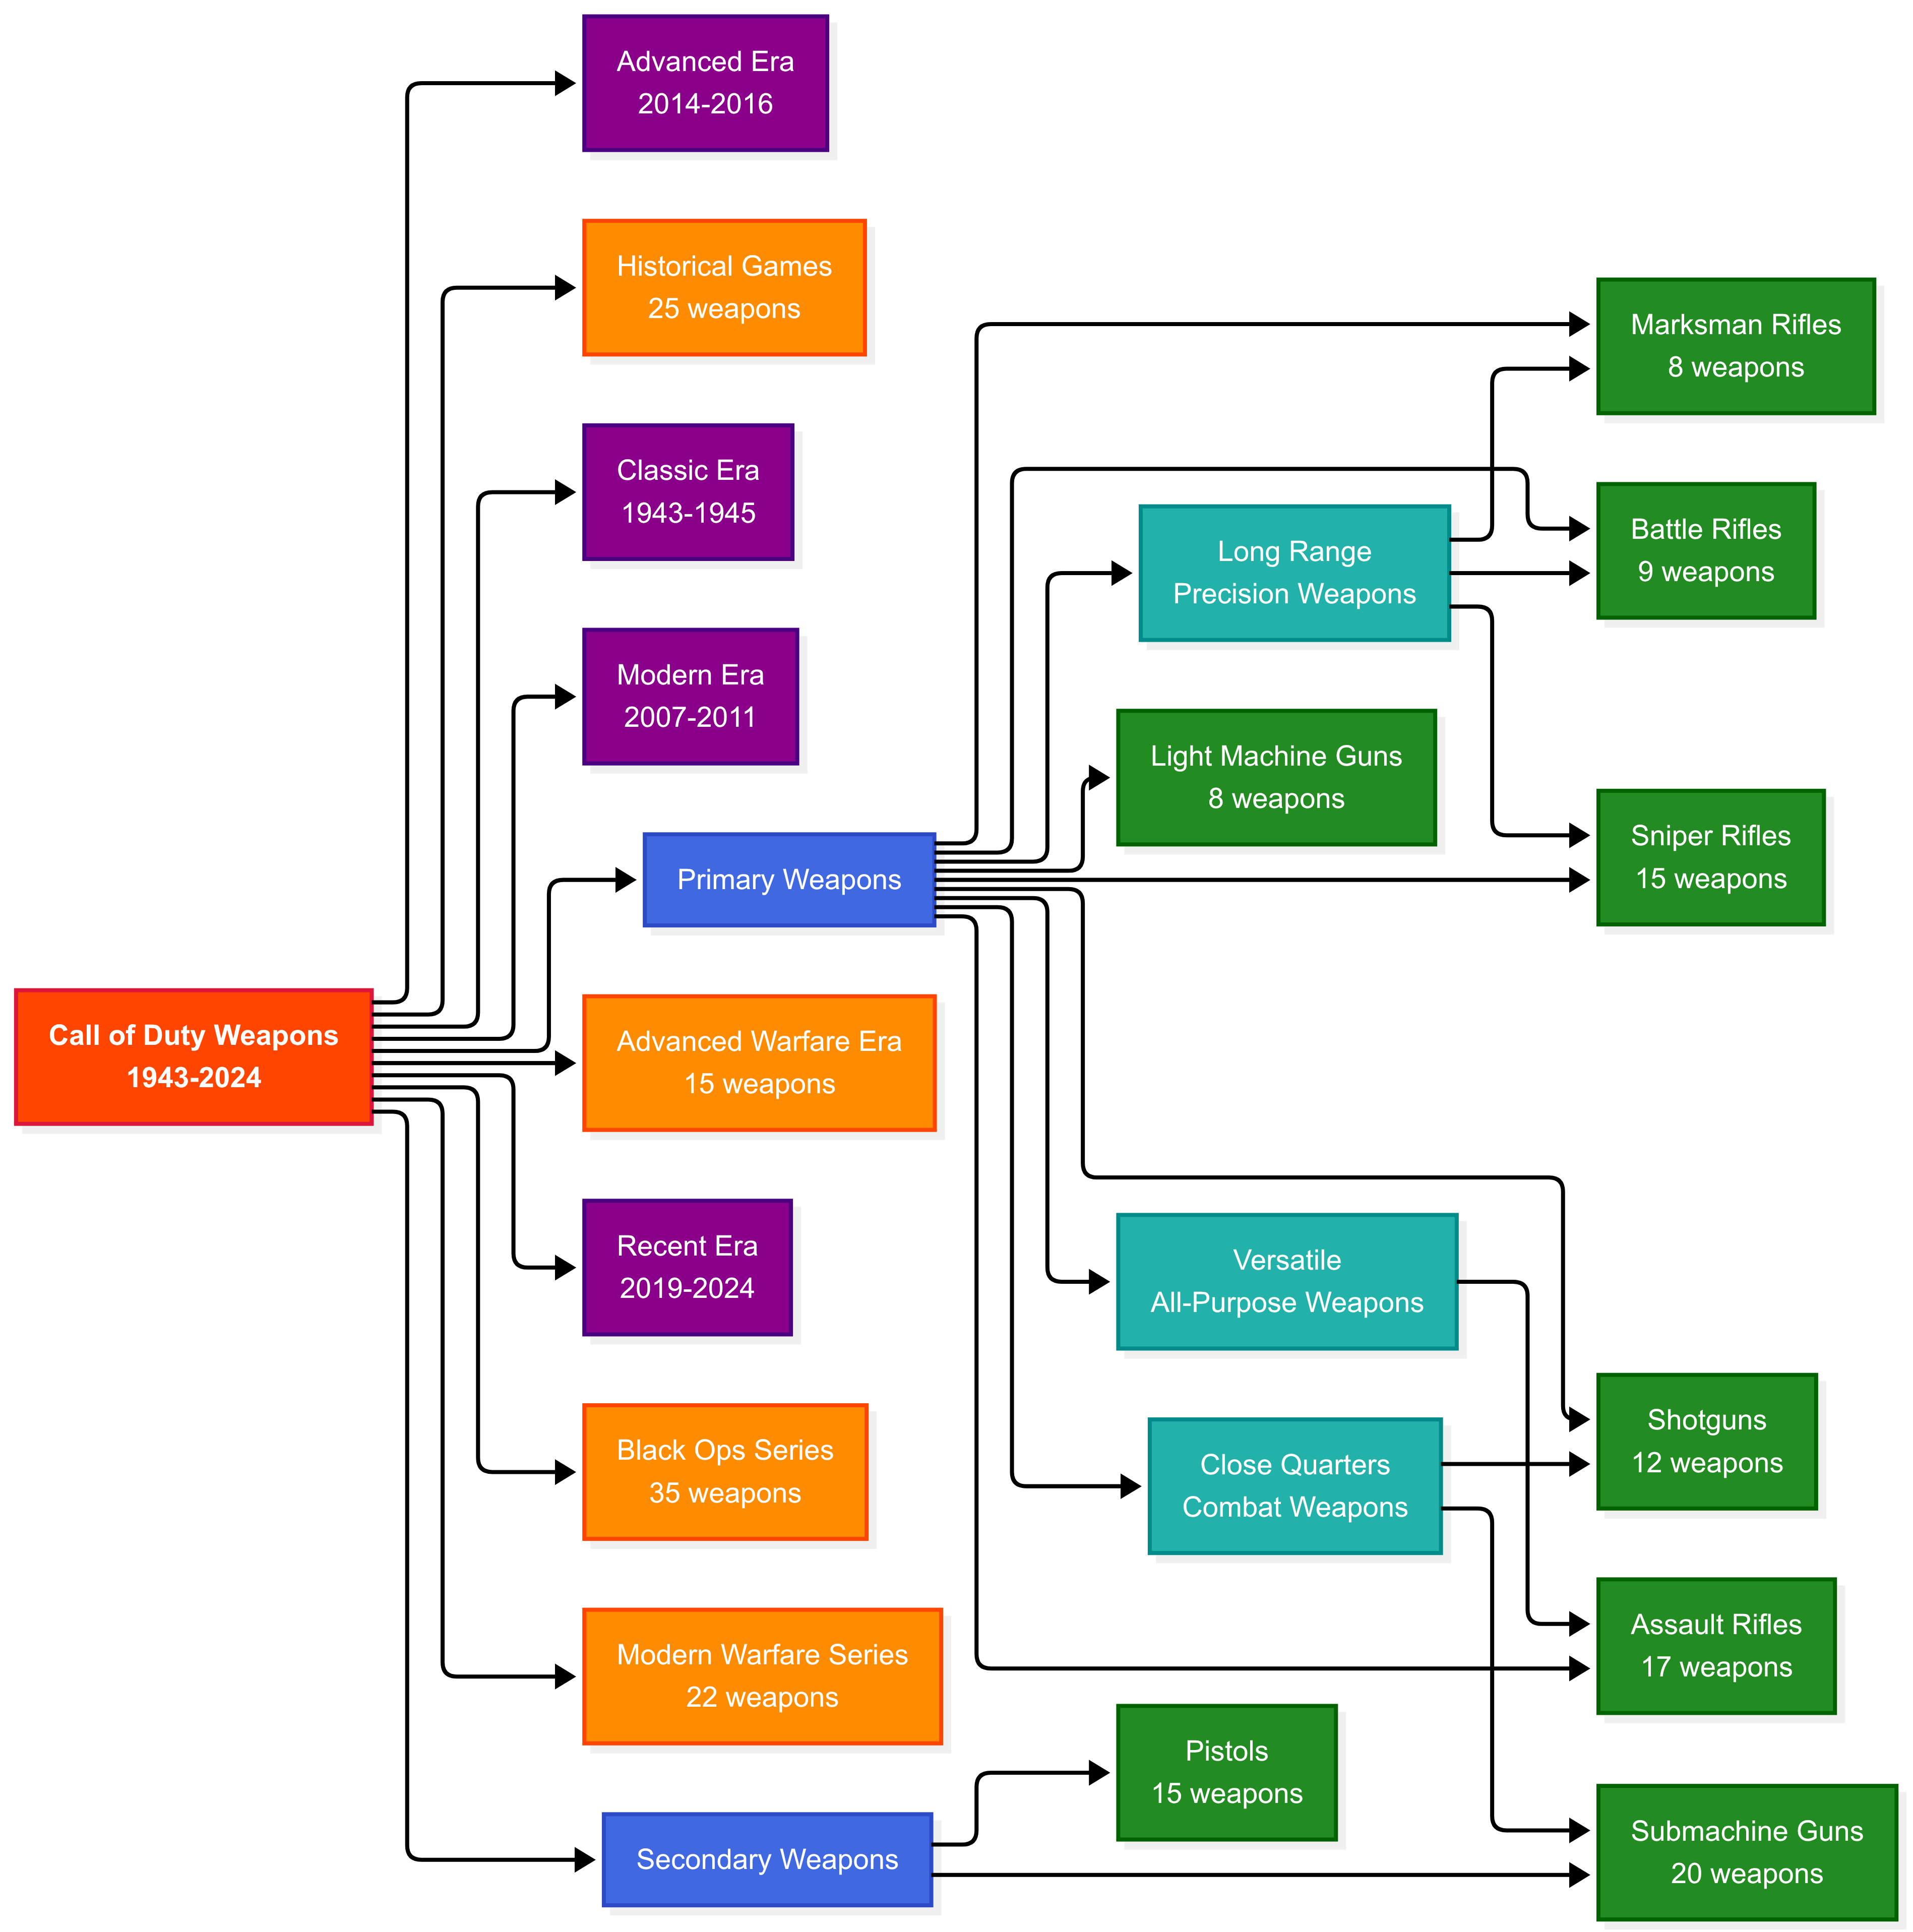
\includegraphics[width=0.9\textwidth]{../diagrams/weapon-type-family-classification-vertical.png}
    \caption{Weapon Type Family Classification Structure}
\end{figure}

\subsection{Weapon Progression System}

The progression system implements complex unlock chains where weapons are interconnected through prerequisite relationships, enabling recursive analysis of progression paths as demonstrated in Figure 3.

\begin{figure}[H]
    \centering
    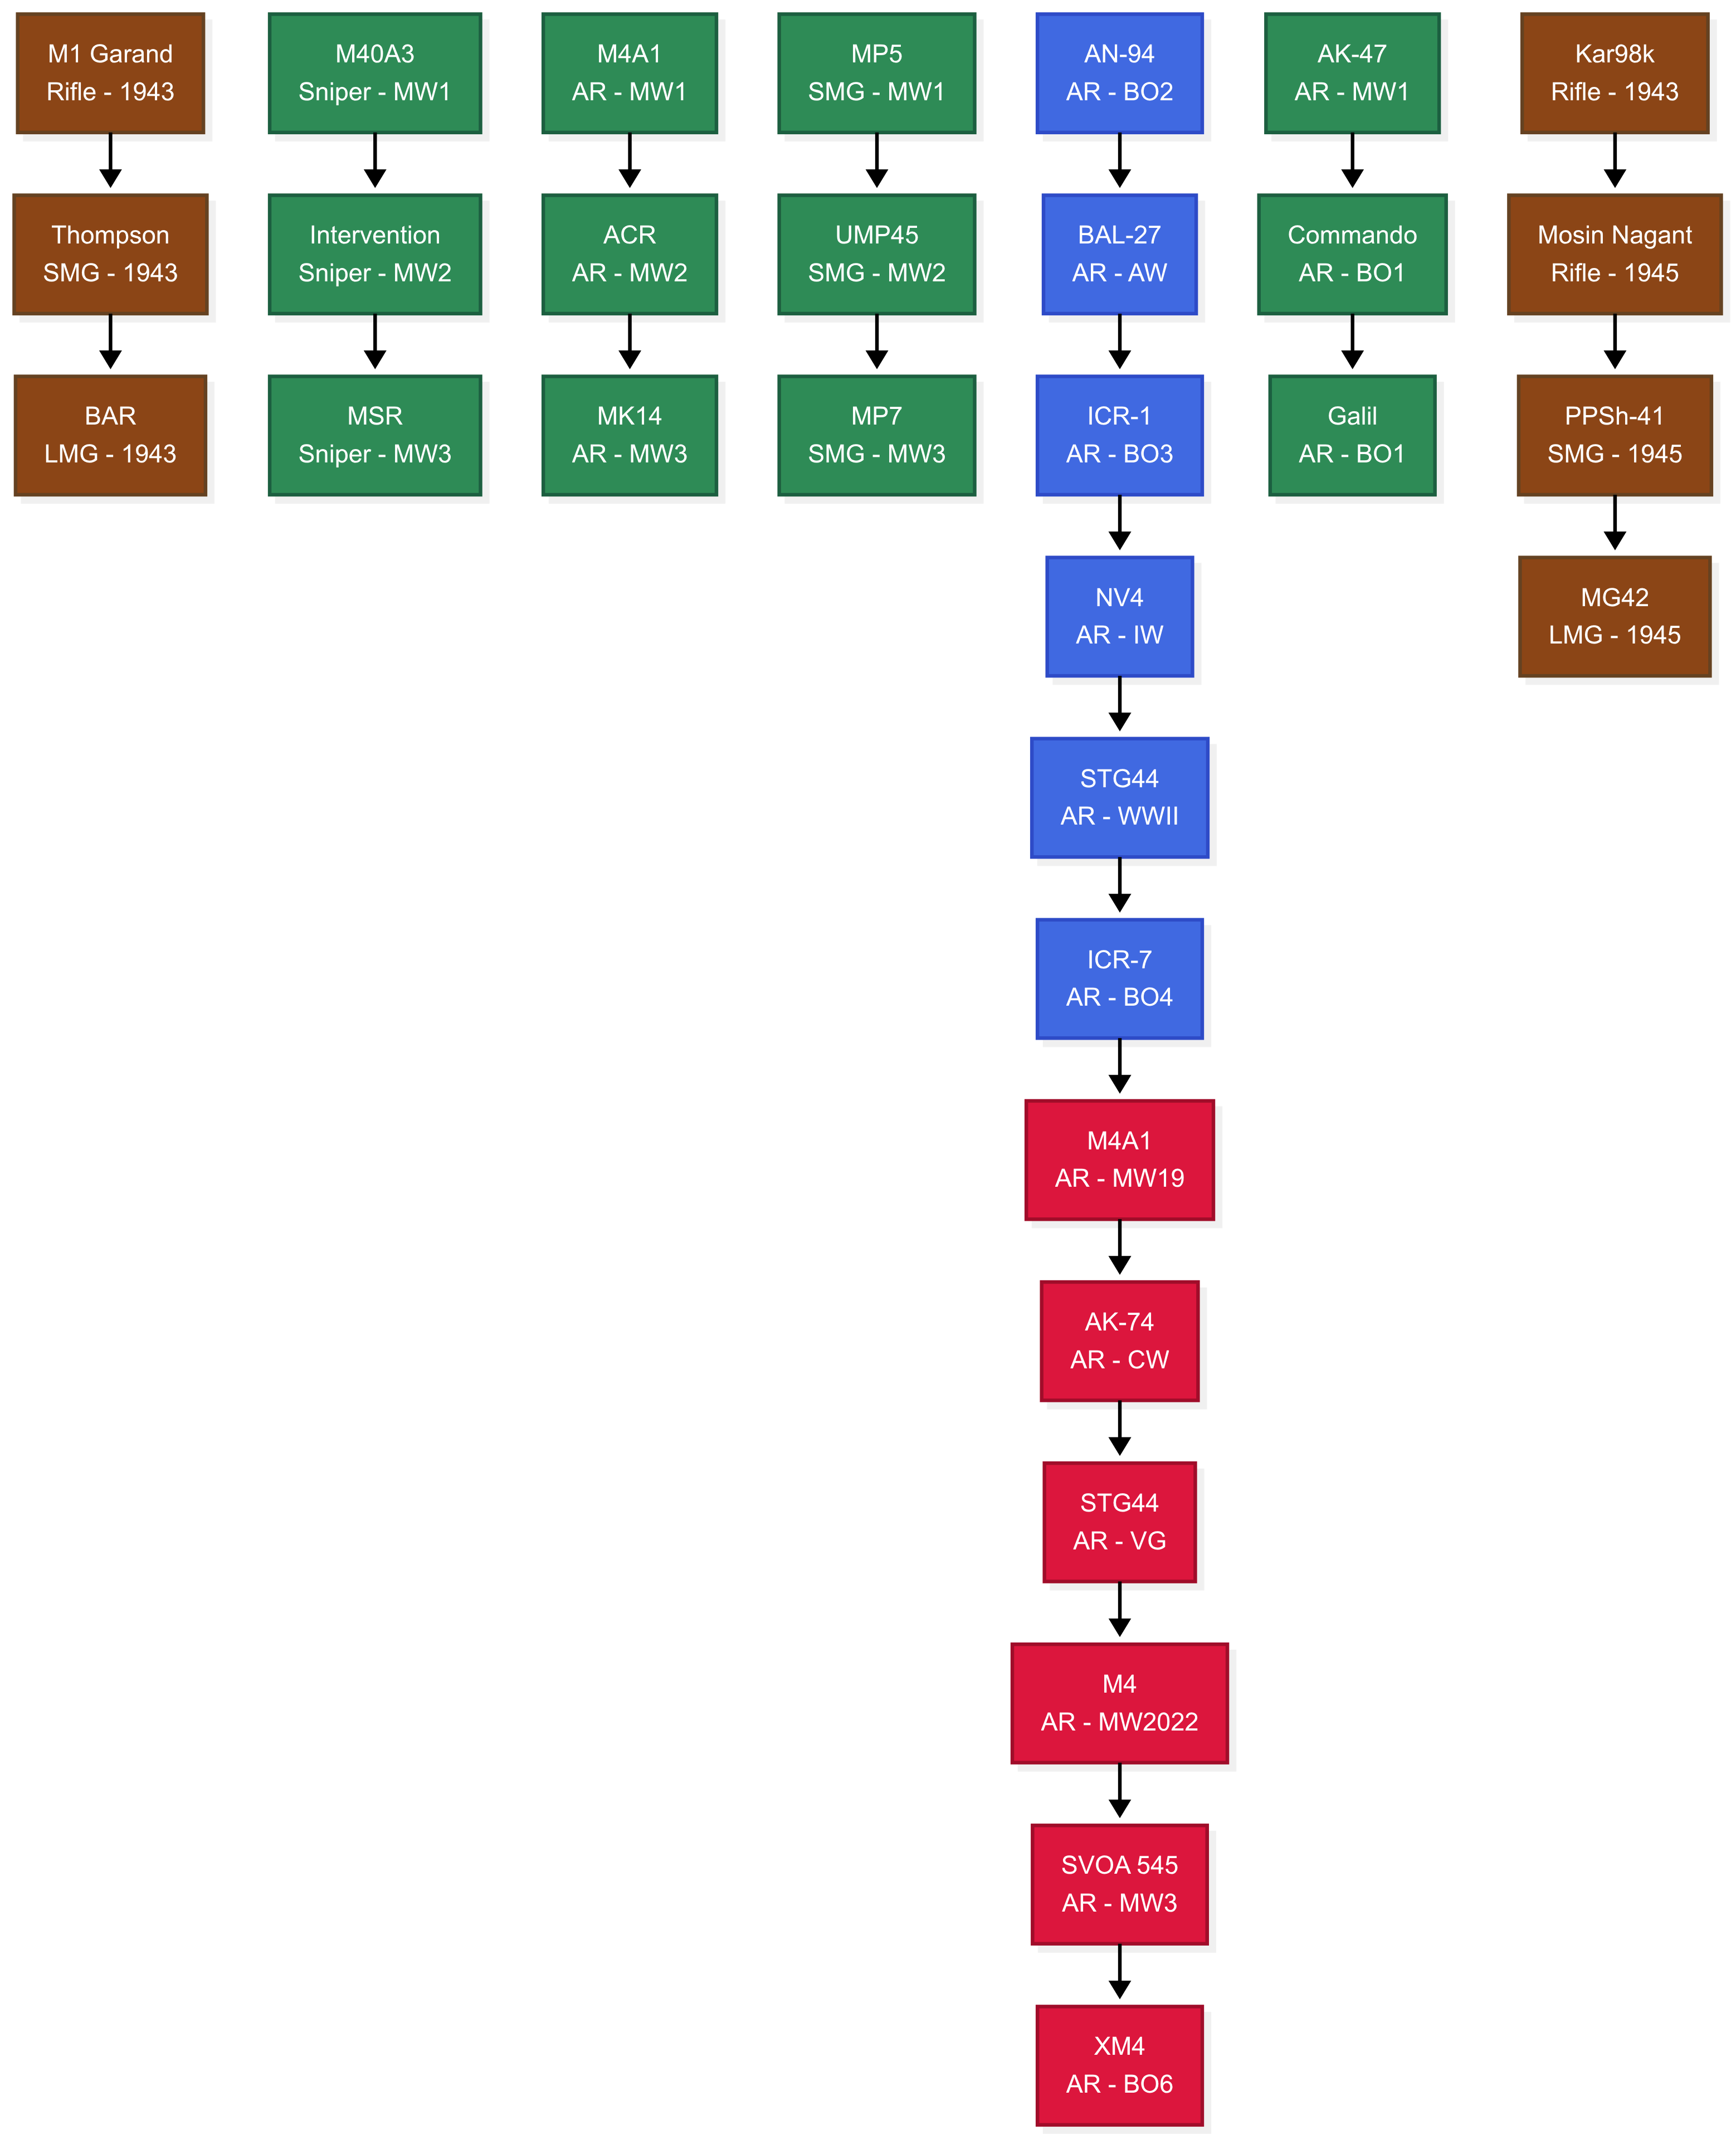
\includegraphics[width=0.9\textwidth]{../diagrams/weapon-progression-family-tree-vertical.png}
    \caption{Weapon Progression Family Tree and Unlock Chains}
\end{figure}

\subsection{Attachment Progression Framework}

The attachment system features its own progression hierarchy where advanced attachments require unlocking prerequisite attachments, creating complex dependency chains illustrated in Figure 4.

\begin{figure}[H]
    \centering
    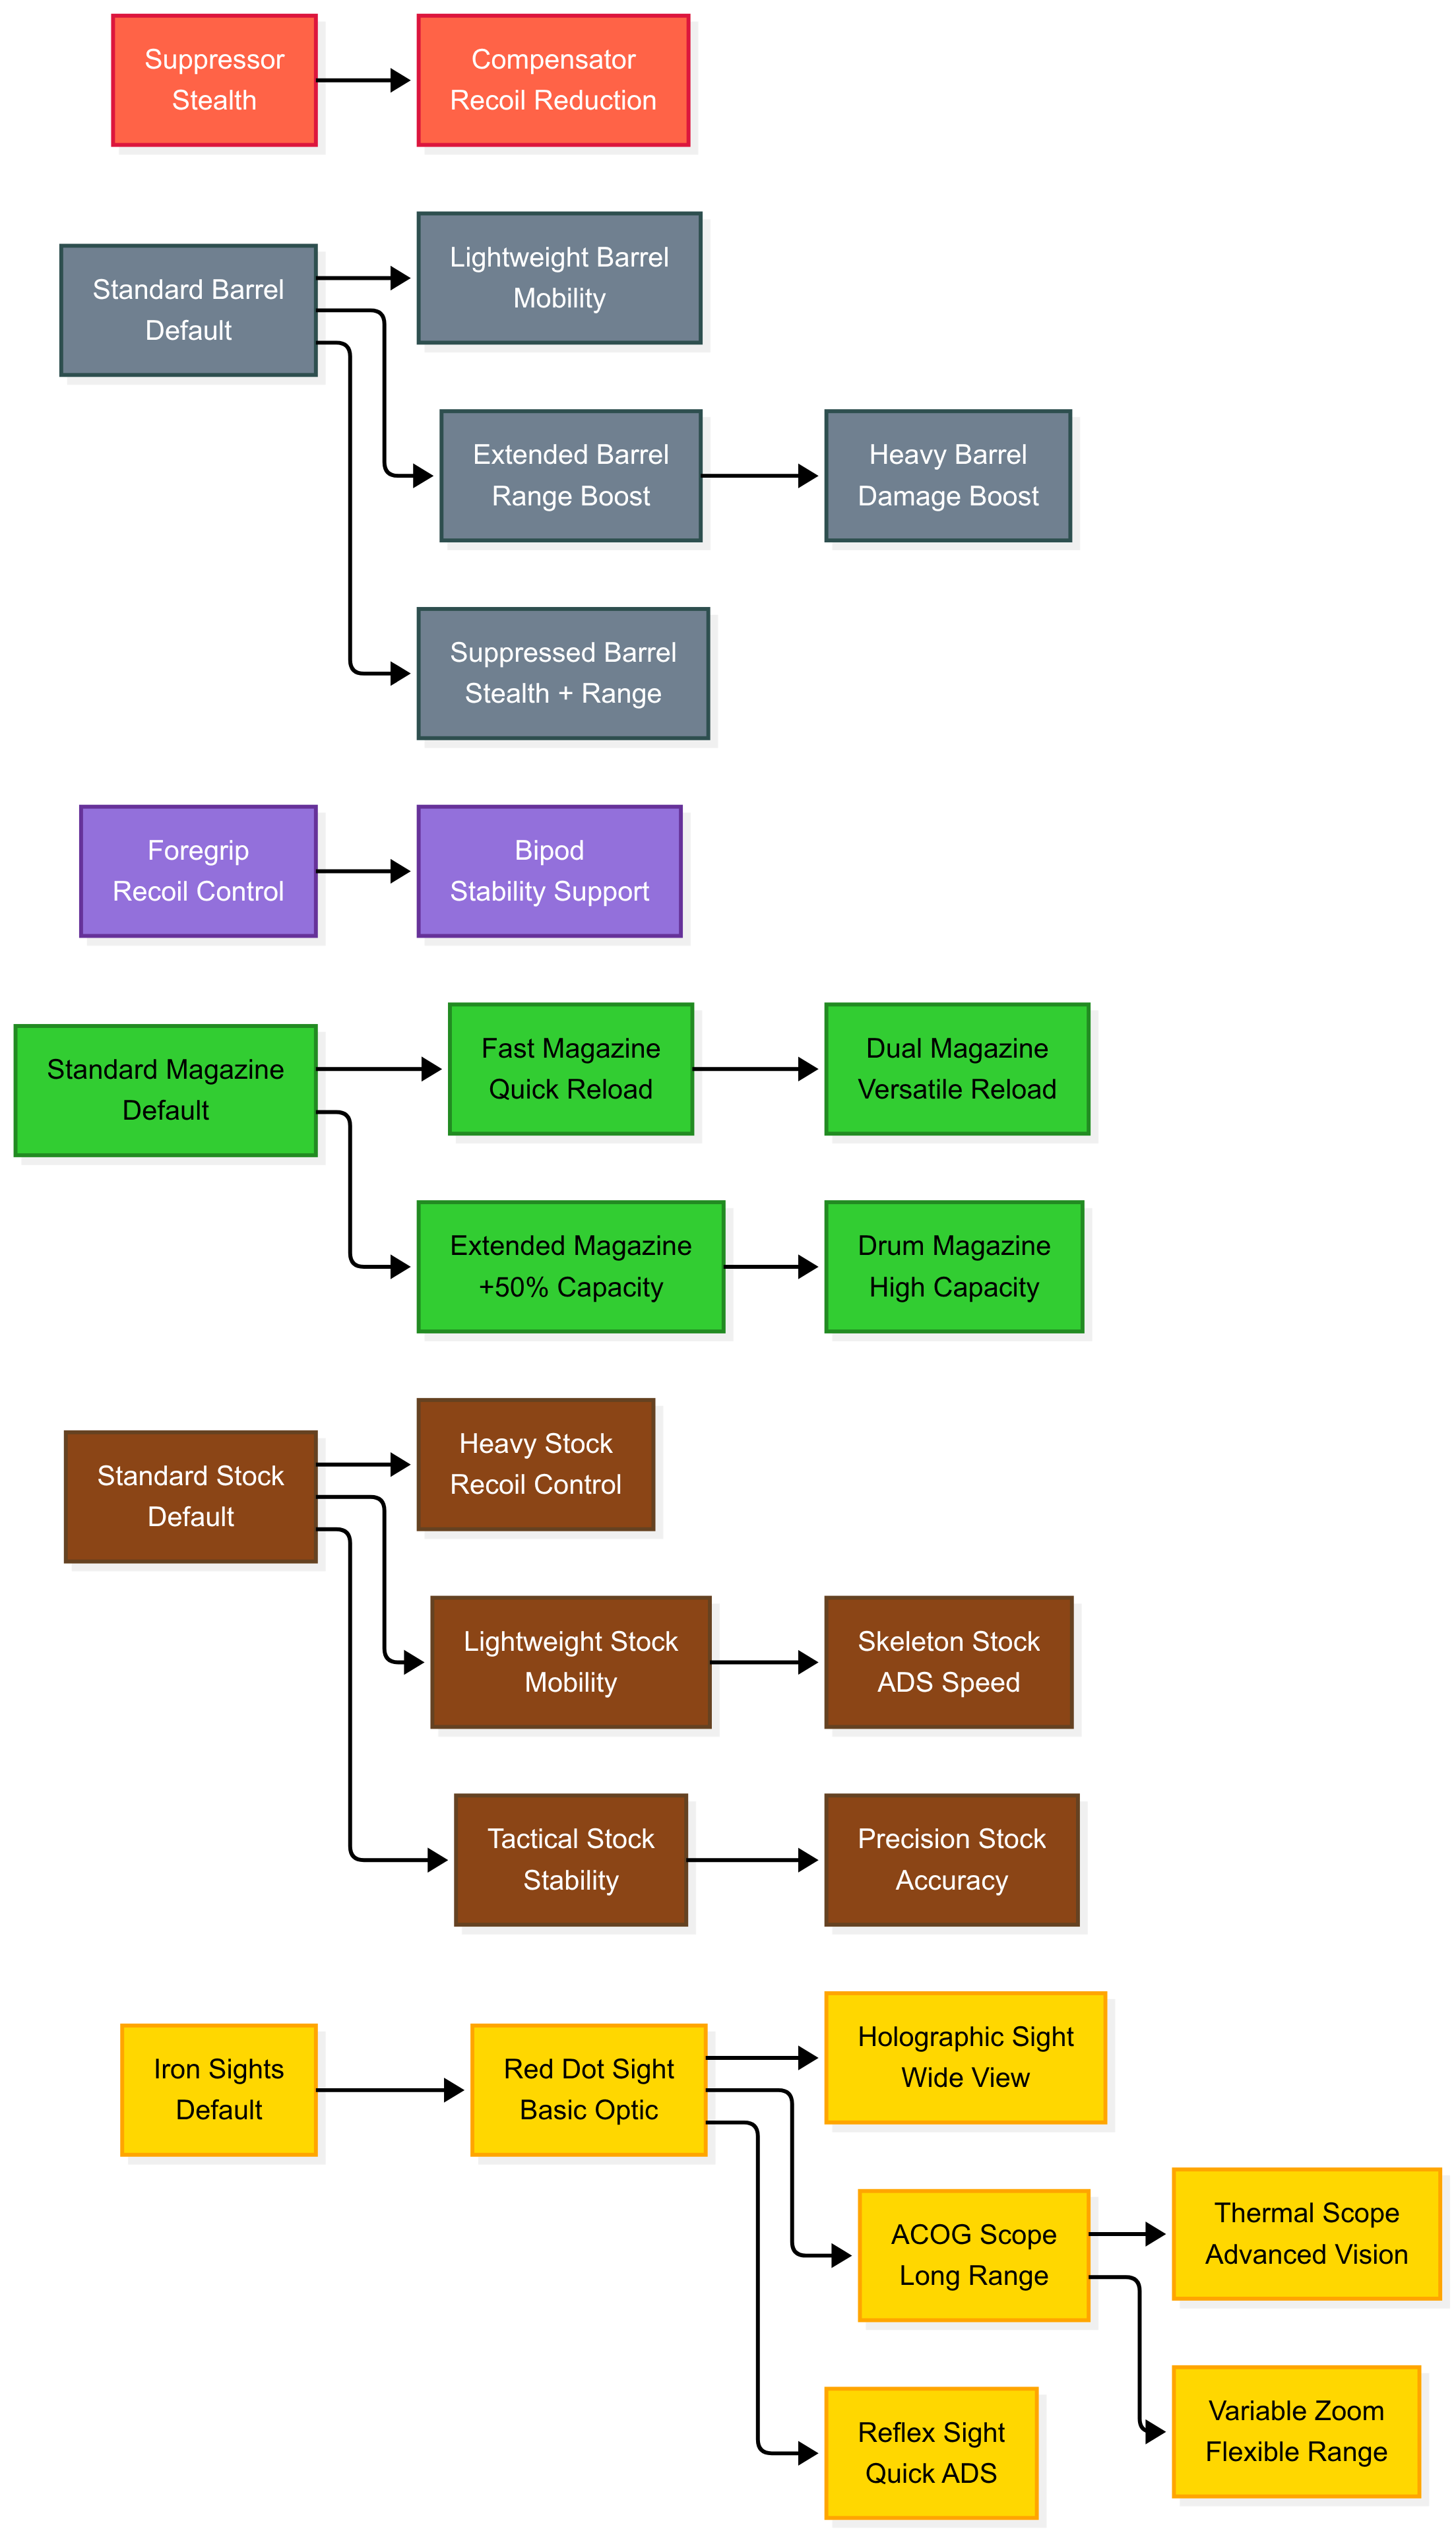
\includegraphics[width=0.9\textwidth]{../diagrams/attachment-progression-family-tree-vertical.png}
    \caption{Attachment Progression Family Tree and Dependencies}
\end{figure}

\subsection{Game Mechanics Evolution}

The evolution of game mechanics across different Call of Duty titles shows the progression of complexity and feature development over the franchise's history, as visualized in Figure 5.

\begin{figure}[H]
    \centering
    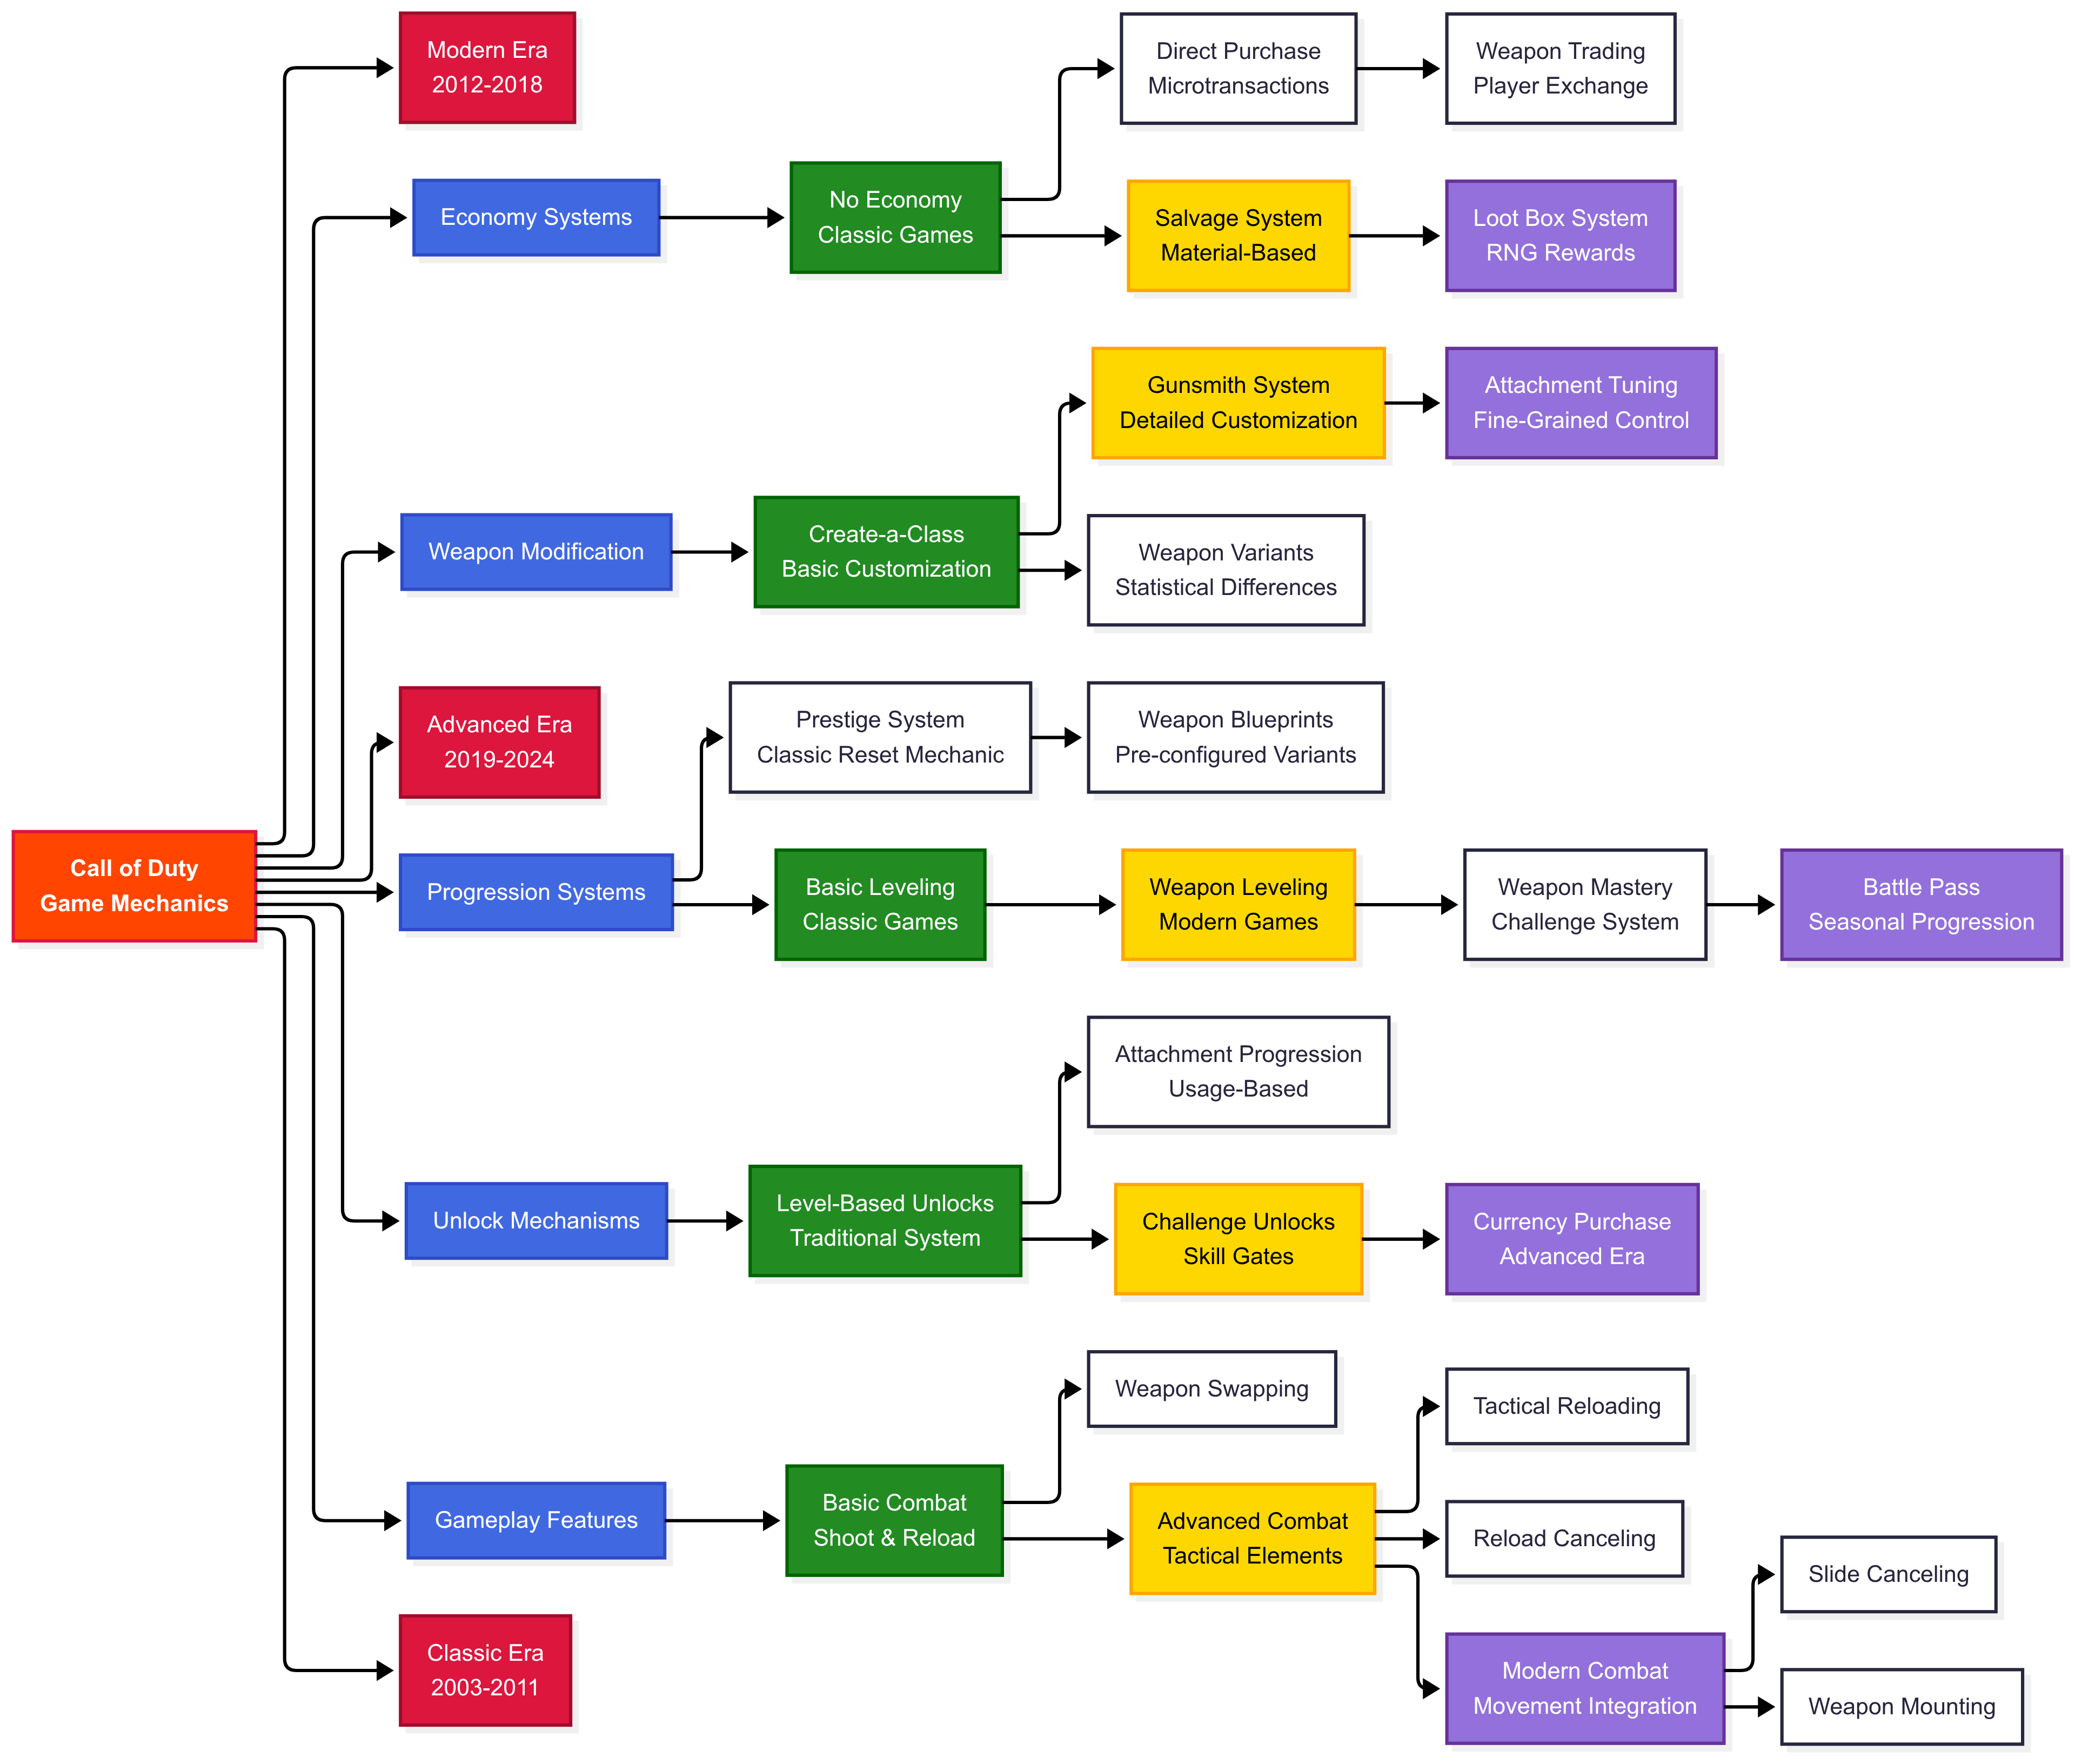
\includegraphics[width=0.9\textwidth]{../diagrams/game-mechanics-evolution-tree-vertical.png}
    \caption{Game Mechanics Evolution Across Call of Duty Titles}
\end{figure}

\section{Sample Input/Output}

\subsection{Basic Weapon Queries}

\textbf{Query}: Find all assault rifles in the knowledgebase
\begin{lstlisting}[language=Prolog]
?- gun_type(assault_rifle, Gun).
\end{lstlisting}

\textbf{Output}:
\begin{lstlisting}
Gun = m4a1 ;
Gun = ak47 ;
Gun = acr ;
Gun = commando ;
Gun = galil ;
Gun = an94 ;
Gun = bal27 ;
Gun = icr1 ;
Gun = nv4 ;
Gun = stg44 ;
Gun = icr7 ;
Gun = m4a1_mw19 ;
Gun = ak74 ;
Gun = stg44_vg ;
Gun = m4_mw2 ;
Gun = svoa_545 ;
Gun = xm4.
\end{lstlisting}

\subsection{Advanced Recursive Queries}

\textbf{Query}: Check if M4A1 can eventually unlock XM4 through progression
\begin{lstlisting}[language=Prolog]
?- can_unlock_eventually(m4a1, xm4).
\end{lstlisting}

\textbf{Output}:
\begin{lstlisting}
true.
\end{lstlisting}

\textbf{Query}: Get the complete unlock chain starting from M4A1
\begin{lstlisting}[language=Prolog]
?- unlock_chain(m4a1, Chain).
\end{lstlisting}

\textbf{Output}:
\begin{lstlisting}
Chain = [m4a1, acr, mk14].
\end{lstlisting}

\subsection{Complex Analysis Queries}

\textbf{Query}: Find weapons suitable for stealth builds
\begin{lstlisting}[language=Prolog]
?- stealth_build(Gun, Attachments),
   length(Attachments, Count),
   Count > 0.
\end{lstlisting}

\textbf{Output}:
\begin{lstlisting}
Gun = m4a1,
Attachments = [suppressor],
Count = 1 ;

Gun = mp5,
Attachments = [suppressor],
Count = 1 ;

Gun = m40a3,
Attachments = [suppressor],
Count = 1.
\end{lstlisting}

\textbf{Query}: Calculate progression depth for XM4
\begin{lstlisting}[language=Prolog]
?- progression_depth(xm4, Depth).
\end{lstlisting}

\textbf{Output}:
\begin{lstlisting}
Depth = 6.
\end{lstlisting}

\subsection{Statistical Analysis}

\textbf{Query}: Find the most common weapon type
\begin{lstlisting}[language=Prolog]
?- most_common_weapon_type(Type).
\end{lstlisting}

\textbf{Output}:
\begin{lstlisting}
Type = assault_rifle.
\end{lstlisting}

\textbf{Query}: Count weapons by type
\begin{lstlisting}[language=Prolog]
?- count_weapons_by_type(assault_rifle, Count).
\end{lstlisting}

\textbf{Output}:
\begin{lstlisting}
Count = 17.
\end{lstlisting}

\subsection{Optimization Queries}

\textbf{Query}: Find optimal damage build for AK-47
\begin{lstlisting}[language=Prolog]
?- optimal_damage_build(ak47, Attachments).
\end{lstlisting}

\textbf{Output}:
\begin{lstlisting}
Attachments = [heavy_barrel, compensator].
\end{lstlisting}

\subsection{Era-Based Classification Queries}

\textbf{Query}: Find all weapons from the modern era
\begin{lstlisting}[language=Prolog]
?- modern_era_guns(Gun).
\end{lstlisting}

\textbf{Output}:
\begin{lstlisting}
Gun = m4a1 ;
Gun = ak47 ;
Gun = mp5 ;
Gun = m249_saw ;
Gun = m40a3 ;
Gun = desert_eagle ;
Gun = w1200 ;
Gun = acr ;
Gun = intervention.
\end{lstlisting}

\subsection{Attachment Compatibility Queries}

\textbf{Query}: Find highly compatible attachments for MP5
\begin{lstlisting}[language=Prolog]
?- highly_compatible_attachments(mp5, Attachment).
\end{lstlisting}

\textbf{Output}:
\begin{lstlisting}
Attachment = suppressor ;
Attachment = extended_mag ;
Attachment = laser_sight.
\end{lstlisting}

\subsection{Weapon Performance Analysis}

\textbf{Query}: Find weapons suitable for close quarters combat
\begin{lstlisting}[language=Prolog]
?- best_close_quarters_weapon(Gun).
\end{lstlisting}

\textbf{Output}:
\begin{lstlisting}
Gun = ppsh_41 ;
Gun = mp5 ;
Gun = ump45 ;
Gun = mp7.
\end{lstlisting}

\textbf{Query}: Find well-supported weapons (3+ attachments)
\begin{lstlisting}[language=Prolog]
?- well_supported_weapons(Gun).
\end{lstlisting}

\textbf{Output}:
\begin{lstlisting}
Gun = m4a1 ;
Gun = ak47 ;
Gun = mp5 ;
Gun = intervention ;
Gun = m249_saw.
\end{lstlisting}

\subsection{Game Mechanics Queries}

\textbf{Query}: Find progression-related game mechanics
\begin{lstlisting}[language=Prolog]
?- progression_mechanics(Mechanic).
\end{lstlisting}

\textbf{Output}:
\begin{lstlisting}
Mechanic = weapon_leveling ;
Mechanic = prestige_system ;
Mechanic = weapon_mastery ;
Mechanic = battle_pass ;
Mechanic = weapon_blueprints ;
Mechanic = camo_challenges.
\end{lstlisting}

\section{Conclusion and Challenges}

\subsection{Project Achievements}

This Call of Duty Weapon Knowledgebase successfully demonstrates Prolog's
capabilities for modeling complex, interconnected systems. The implementation
incorporates sophisticated recursive algorithms, multi-dimensional
classification systems, and optimization frameworks that showcase advanced
logical programming concepts.

\textbf{Key Accomplishments}:
\begin{enumerate}
    \item \textbf{Comprehensive Data Model}: Successfully modeled 121 weapons, 49 attachments, and 26 game mechanics spanning 21 years of gaming history.
    \item \textbf{Advanced Recursive Systems}: Implemented sophisticated recursive rules for progression analysis and optimization algorithms.
    \item \textbf{Multi-Dimensional Analysis}: Created flexible classification systems for era, type, role, and performance analysis.
    \item \textbf{Practical Applications}: Developed optimization algorithms providing real-world weapon build recommendations.
\end{enumerate}

\subsection{Technical Challenges and Solutions}

\textbf{Recursive Query Optimization}: Initial performance issues with deep unlock trees were resolved through tail-recursive optimizations and memoization techniques.

\textbf{Attachment Compatibility Matrix}: The complex relationship between 121 weapons and 49 attachments was managed using a 1-5 rating system for nuanced compatibility assessment.

\textbf{Era Classification Ambiguity}: Overlapping game characteristics were handled through flexible classification rules allowing multiple era memberships.

\textbf{Query Performance}: Complex recursive operations were optimized through strategic fact ordering and rule optimization.

\subsection{Educational Value and Future Work}

This project demonstrates Prolog's effectiveness for knowledge representation,
recursive logic implementation, expert system development, and data pattern
extraction. Future enhancements could include machine learning integration for
predictive recommendations, performance optimization through constraint logic
programming, web interface development, and real-time API connections for
dynamic updates.

The project showcases that Prolog remains highly relevant for modern
knowledge-based systems, particularly in domains involving complex
relationships and logical inference. This knowledgebase serves as both an
educational resource and a foundation for future gaming analytics research.

\end{document}
